\subsection{Datasets}
\begin{table}[h]
    \center
    \begin{tabular}{r c c}
        \toprule
        Dataset & Number of tokens & Number of types \\
        \midrule
  English verbs & 113k & 7k \\
        Russian adjectives & 280k & 30k \\
        \bottomrule
    \end{tabular}
    \caption{Corpus and vocabulary size of the two datasets used for evaluation}
    \label{tab:datasets}
\end{table}

Our first goal is to prove that the different parametrizations of the model perform equally well. To do so, we attempt to replicate previous work by using the dataset from \cite{goldwater2011}. This dataset is composed of all the verbs from the Penn treebank corpus, which are decomposed into a prefix, suffix pair using a small set of rules. English verbs have only a few possible endings ($\emptyset$, -e, -ed, ing, -s, -en \dots) but there is no clear gold segmentation for irregular verbs (should the form \textit{said} be analyzed as \textit{sai+d} or \textit{said}+$\emptyset$ ?). To obtain more empirical evidence of the validity of our approach, we also consider a larger dataset that we create by sampling Russian adjectives from a tagged corpus of news articles. In this case, the segmentation is fully unambiguous but the number of possible suffixes for each word is much larger: English verbs have only three forms (present, past, progressive) whereas Russian adjectives can be found in up to 24 different forms (3 genders + 2 numbers * 6 cases). The size of these two datasets are given in Table~\ref{tab:datasets}.

\subsection{Experiments and discussion}

\begin{table}[h]
    \center
    \begin{tabular}{r c c c c}
        \toprule
        Model & \multicolumn{2}{c}{Token accuracy} & \multicolumn{2}{c}{Type accuracy} \\
        \cmidrule(r){2-3} \cmidrule(r){4-5}
        & EN & RU & EN & RU \\
        \midrule
        Baseline & 79.3 $\pm$ 3.2 & 99.4 & 77.1 $\pm$ 0.3 & 96.1 \\
          Serial & 82.6 $\pm$ 1.8 & 99.4 & 77.6 $\pm$ 0.1 & 96.2 \\
        Parallel & 84.1 $\pm$ 0.3 & 99.5 & 77.1 $\pm$ 0.2 & 96.1 \\
        \bottomrule
    \end{tabular}
    \caption{Accuracy of the segmentations for the two datasets -- English accuracies are averaged over the last 1000 iterations}
    \label{tab:accuracy}
\end{table}

We run the three versions of the model on these two datasets to compare their performance. We set the parameters to $\alpha = 10^{-6}, \alpha_p = \alpha_s = 10^{-3}$ according to the discussion in \cite{goldwater2011} and let the Gibbs sampler run for 10,000 iterations. The parallel model is run with 4 processes. Unsurprisingly, we obtain very close accuracies for all models (Table~\ref{tab:accuracy}), with the exception of token accuracies in English which vary a lot because of the uncertainity of the irregular forms (the top 10 forms \textit{is/said/was/be/are/has/have/says/were/had} account for 30\% of the tokens and are irregular).

In terms of speed, the baseline and the serial models are comparable for a fixed number of iterations, and the parallel model is 30\% faster than the serial model with 4 processors. We expect the time difference to be even greater for larger corpora, as the time spent in the message passing steps is currently relatively high (20\% of the total time).

\begin{figure}[h]
    \center
    \begin{subfigure}{0.48\textwidth}
        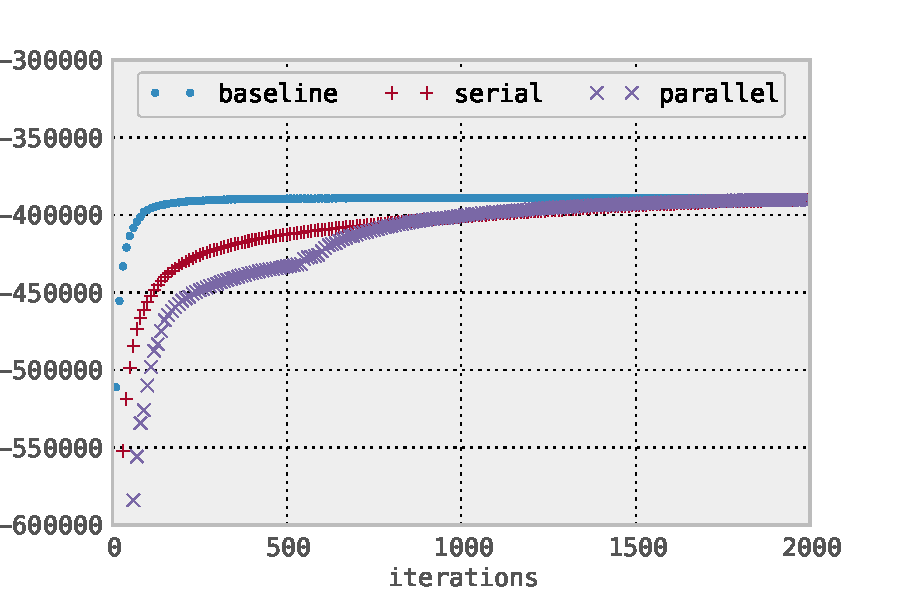
\includegraphics[width=\textwidth]{fig/base_ll}
        \subcaption{Log-likelihood of the base distribution}
        \label{fig:ll_base}
    \end{subfigure}
    \begin{subfigure}{0.48\textwidth}
        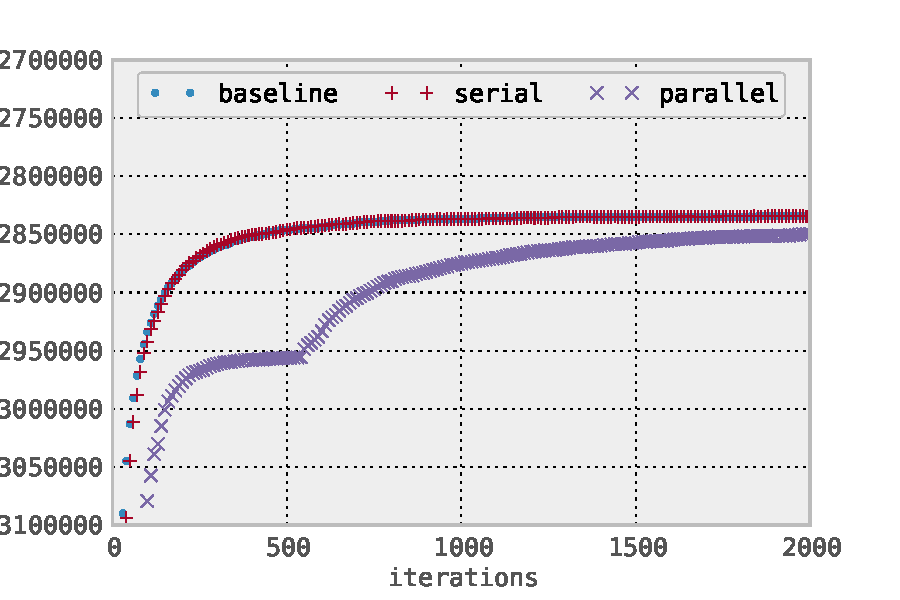
\includegraphics[width=\textwidth]{fig/crp_ll}
        \subcaption{Log-likelihood of the CRP}
        \label{fig:ll_crp}
    \end{subfigure}
    \caption{Log-likelihood of the three models (baseline: \S\ref{sec:existing-models}, serial: \S\ref{sec:dpmm}, parallel: \S\ref{sec:parallel-goldwater}) -- Russian dataset}
    \label{fig:ll}
\end{figure}


To further understand the differences between the three proposed samplers, we consider the evolution of the log-likelihood of the models over time when trained on the Russian dataset (Figure~\ref{fig:ll}). The first thing to notice (\ref{fig:ll_base}) is that the serial model takes longer to converge than the baseline model. There is a simple explanation for this: the base distribution is not collapsed anymore, and although the CRP has an identical behavior (\ref{fig:ll_crp}), this affects the full model convergence. The second striking difference is between the serial and the parallel model likelihoods: while they are close, the parallel model suffers from some delay due to the random table assignment to processors. We observe after 500 iterations a successful Metropolis-Hastings redistribution step of the tables that produces a more efficient configuration for the sampler.

\begin{figure}[h]
    \center
    \begin{subfigure}{0.48\textwidth}
        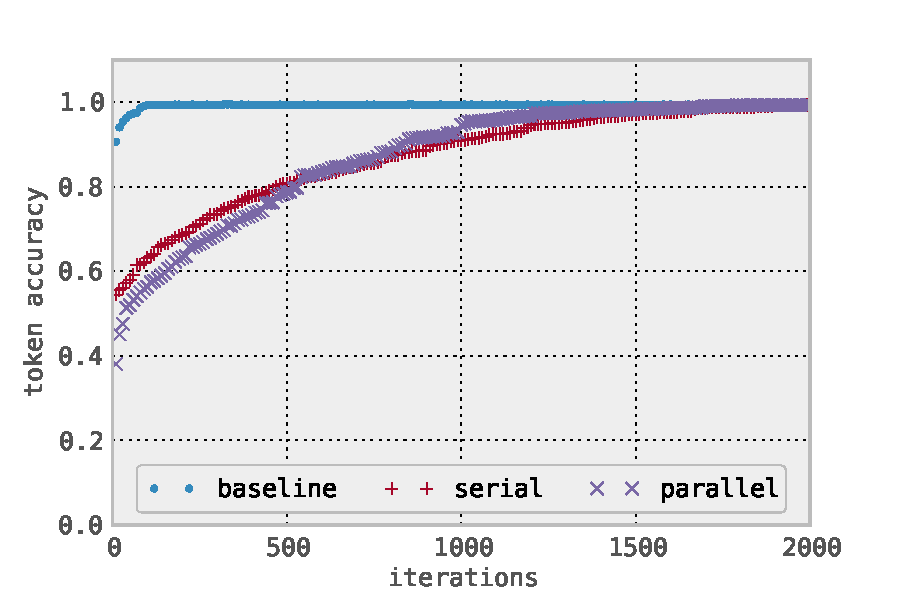
\includegraphics[width=\textwidth]{fig/token_acc}
        \subcaption{Token accuracy}
        \label{fig:token_acc}
    \end{subfigure}
    \begin{subfigure}{0.48\textwidth}
        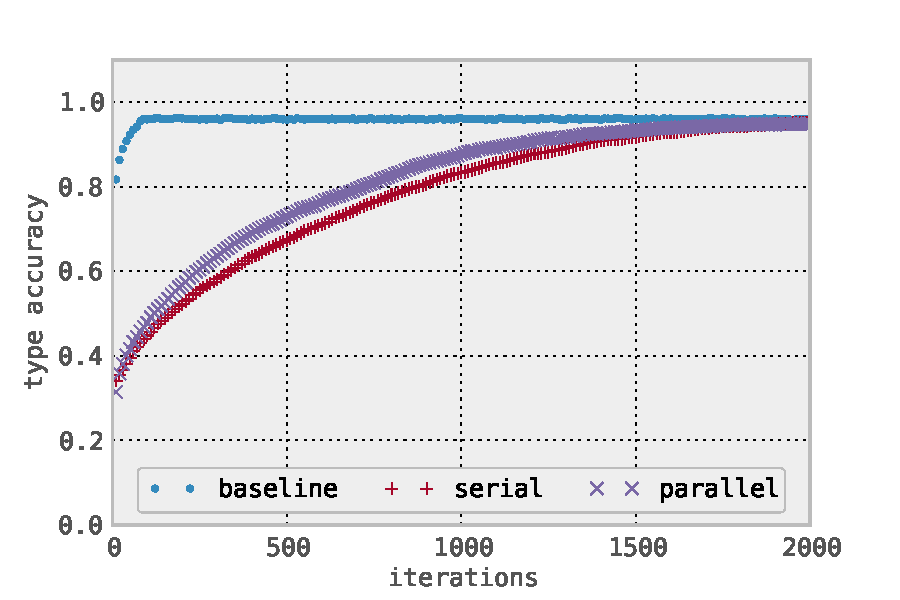
\includegraphics[width=\textwidth]{fig/type_acc}
        \subcaption{Type accuracy}
        \label{fig:type_acc}
    \end{subfigure}
    \caption{Accuracies of the three models (baseline: \S\ref{sec:existing-models}, serial: \S\ref{sec:dpmm}, parallel: \S\ref{sec:parallel-goldwater}) -- Russian dataset}
    \label{fig:acc}
\end{figure}

However, looking at the likelihood of these models does not tell us how long it takes to reach a configuration which produces accurate analyses. In Figure~\ref{fig:acc}, we plot the evolution of the accuracy as a function of the number of iterations, and obtain an expected result: not collapsing the base has a negative effect on the time taken to reach the peak accuracy. However, the role of the CRP is relatively minor and the difference of convergence behavior observed previously when comparing the serial and the parallel models seems to have no effect here.

We can therefore summarize these experiments simply by concluding that although the parallel version is as exact as the serial version while being faster, both of these versions suffer from the theorical requirement that the base be uncollapsed.
